\documentclass[letterpaper, 10 pt, conference]{ieeeconf}  % Comment this line out if you need a4paper
\usepackage{amsmath} 
\usepackage{amssymb} 

\newcommand{\proj}{\mathcal{P}}
\newcommand{\backproj}{\mathcal{Q}}

\usepackage{ltl} 

\usepackage[vlined]{algorithm2e}

\usepackage{color}
\usepackage{subfig}
\usepackage{tikz}
\usepackage{hyperref}
\usetikzlibrary{arrows,fit,shapes,automata}
\usetikzlibrary{positioning,fit,calc,shapes}
\usetikzlibrary{decorations.fractals}
\usetikzlibrary{decorations.markings}

\newcommand{\Rayna}[1]{{\textcolor{magenta}{ \textbf{Rayna:} #1 $\spadesuit$ }}}
\newcommand{\Suda}[1]{{\textcolor{blue}{ \textbf{Suda:} #1 $\spadesuit$ }}}
\newcommand{\Ufuk}[1]{{\textcolor{red}{ \textbf{Ufuk:} #1 $\spadesuit$ }}}
\newcommand{\todo}[1]{{\textcolor{red}{TODO:} #1}}
%\newcommand{\comment}[1]{}

\newtheorem{example}{Example}
\newtheorem{theorem}{Theorem}
%\newcommand*{\qed}{\hfill\ensuremath{\blacksquare}}

\newcommand{\init}{\mathsf{init}}
\newcommand{\belief}{\mathsf{belief}}
\newcommand{\abstr}{\mathsf{abstract}}
\newcommand{\vis}{\mathit{vis}}
\newcommand{\succs}{\mathit{succ}}
\newcommand{\beliefs}{\mathcal{P}(L_t)}

\newcommand{\Surveillance}{\mathsf{Surveillance}}
\newcommand{\beliefF}{\mathit{belief}}

\newcommand{\states}{S}
\newcommand{\trans}{T}
%\newcommand{\part}{\mathcal{Q}}

\newcommand{\post}{\mathit{succ}_t}

\newcommand{\outcome}{\mathit{outcome}}
\newcommand{\counterex}{\mathcal{C}}

\newcommand{\bools}{\mathbb{B}}
\newcommand{\true}{\mathit{true}}
\newcommand{\false}{\mathit{false}}
\newcommand{\nats}{\mathbb{N}}

\newcommand{\SP}{\mathcal{SP}}
\newcommand{\AP}{\mathcal{AP}}


\newcommand{\design}{\mathcal{D}}
\newcommand{\proc}{\mathcal{P}}
\newcommand{\Proc}{\mathit{Agts}}
\newcommand{\shield}{\mathcal{S}}
\newcommand{\game}{\mathcal{G}}
\newcommand{\gstates}{S}
\newcommand{\ginit}{s_0}
\newcommand{\buchi}{B\"uchi\xspace}
\newcommand{\Traces}{\mathsf{Traces}}
\newcommand{\Win}{\mathsf{Win}}

\newcommand{\spec}{\varphi}
\newcommand{\lang}{L}
\newcommand{\langset}{\mathcal{L}}
\newcommand{\widx}{\mathsf{WIdx}}
\newcommand{\natsII}{\mathbb{N}^{\infty}}
\newcommand{\enats}{\overline{\mathbb{N}}}
\newcommand{\inp}{\textit{I}}
\newcommand{\out}{\textit{O}}


\newcommand{\Acc}{\mathsf{Acc}}
\newcommand{\Val}{\mathsf{Val}}

\newcommand{\alphabet}{\Sigma}
\newcommand{\ialphabet}{\Sigma_\inp}
\newcommand{\oalphabet}{\Sigma_\out}
\newcommand{\ialphabeti}{\Sigma_{I,i}}
\newcommand{\oalphabeti}{\Sigma_{O,i}}
\newcommand{\ioalphabet}{\Sigma_{\inp \cup \out}}
\newcommand{\calphabet}{\Sigma_{\inp \cup \out \cup \out'}}

\newcommand{\fwords}[1]{#1^*}
\newcommand{\iwords}[1]{#1^\omega}
\newcommand{\awords}[1]{#1^\infty}

\newcommand{\symb}{\sigma}
\newcommand{\isymb}{\sigma_\inp}
\newcommand{\osymb}{\sigma_\out}

\newcommand{\trace}{\overline\sigma}
\newcommand{\itrace}{\overline\sigma_\inp}
\newcommand{\otrace}{\overline\sigma_\out}

\newcommand{\Deviations}{\mathit{Dev}}
\newcommand{\Blame}{\mathit{Blame}}
\newcommand{\Correct}{\mathit{Mcs}}
\newcommand{\Diff}{\mathit{Diff}}
\newcommand{\DevSet}{\mathit{Dev}}

\newcommand{\comp}{\circ}



   
%\documentclass[a4paper, 10pt, conference]{ieeeconf}      % Use this line for a4 paper

\IEEEoverridecommandlockouts                              % This command is only needed if 
                                                          % you want to use the \thanks command

\overrideIEEEmargins                                      % Needed to meet printer requirements.

%\renewcommand{\baselinestretch}{2}

% See the \addtolength command later in the file to balance the column lengths
% on the last page of the document
\pdfminorversion=4

\title{\LARGE \bf Cool title here}

\author{Author Name$^{1}$ and Author Name$^{2}$ and Author Name$^{1}$ and Author Name$^{2}$ % stops a space
%\thanks{*This work was not supported by any organization}% <-this % stops a space
\thanks{$^{1}$}%
\thanks{$^{2}$}%
}


\begin{document}
\maketitle
\thispagestyle{empty}
\pagestyle{empty}

\begin{abstract}

We consider the problem of maximizing visibility coverage of an environment while satisfying a surveillance requirement, that is, maintain knowledge on the location of a potentially adversarial moving target. Using a level set representation of data and information, we train a convolutional neural network to determine vantage points that maximize visibility. While this method reduces online computation cost, it does not guarantee the surveillance requirement. We represent this requirement as a GR(1) temporal logic formula on a partial-information two player game and synthesize a permissive strategy. 


\end{abstract}


\section{Introduction}

Want to do surveillance. However, it is also important to routinely observe parts of the map that haven't been seen in a while. We combine the two. 

\subsection{Related work}
Other surveillance work, some optimal exploration work. Maybe even some runtime monitoring work


\subsection{Contribution}
A framework to allow for patrolling of a map constrained by a the surveillance requirement on a hostile target. Comes with formal guarantees of correctness as well quantitative guarantees on surveillance. Also efficient exploration. 


\section{Preliminaries}
\label{sec_prel}



\subsubsection{Two-player Games}
%
A two-player game is a tuple $\game = (\gstates,
\ginit, \alphabet, \delta, \Acc)$,
where $\gstates$ is a finite set of states, $\ginit \in \gstates$ is the initial state,
$\delta: \gstates \times \alphabet \rightarrow \gstates$
is a complete transition function, $\Acc: (\gstates \times \alphabet \times \gstates)^\omega \rightarrow \bools$ is a winning condition
and defines the qualitative objective of the game.
%
The game is played  by two players:  the system and the environment. In every state $s\in \gstates$
(starting with $\ginit$), the environment chooses an input
$\isymb \in \ialphabet$, and then the system chooses some output $\osymb \in \oalphabet$. These choices define the next state $s' = \delta(s,(\isymb, \osymb))$, and so on. The resulting (infinite)
sequence $\overline{\pi} = (\ginit,\isymb, \osymb, s_1) (s_1,\isymb, \osymb, s_2) \ldots$ is called a \emph{play}.
A deterministic  \emph{strategy} for the environment is a function
$\rho_e: \gstates^* \rightarrow \ialphabet$.
A nondeterministic \emph{strategy} for the system is a relation $\rho_s:
\gstates^* \times \ialphabet \rightarrow 2^{\oalphabet}$ and a
deterministic  strategy for the system is a function $\rho_s:
\gstates^* \times \ialphabet \rightarrow \oalphabet$.\looseness=-1

A play $\overline{\pi}$ is \emph{won} by the system iff $\Acc(\overline{\pi})=\top$.
 A strategy is \emph{winning} for the system if all plays $\overline{\pi}$ that can be
constructed when defining the outputs using the strategy result in
$\Acc(\overline{\pi})=\top$. The \emph{winning region} $\Win$ is the set of states
from which a winning strategy exists.
A \emph{permissive} winning strategy  $\rho_s:
\gstates^* \times \ialphabet \rightarrow 2^{\oalphabet}$ is a strategy that is not only winning for the system, but also contains all deterministic winning strategies.

A \emph{safety game} defines $\Acc$ via a set $F\subseteq \gstates$ of
safe states: $\Acc(\overline{\pi})=\top$ iff $g_i \in F$ for all $i \geq 0$, i.e., if only safe states are visited in the play $\overline{\pi}$. Otherwise, $\Acc(\overline{\pi})=\bot$.
%If a safety game is won by the system player, then there exists a permissive strategy $\rho_s$ that is \emph{memoryless}, i.e., has the form $\rho_s:
%\gstates \times \ialphabet \rightarrow 2^{\oalphabet}$.
%
The \emph{\buchi} winning condition is $\Acc(\overline{\pi})=\top$ iff $\inf(\overline{\pi})
\cap F \neq \emptyset$, where $F \subseteq Q$ is
the set of accepting states and $\inf(\overline{\pi})$ is the set of states that occur infinitely often in $\overline{\pi}$.
We abbreviate the \buchi condition as $\mathcal{B}(F)$.
A \emph{Generalized Reactivity 1} (GR(1))
acceptance condition is a predicate $\bigwedge_{i=1}^{m} \mathcal{B}(E_{i}) \rightarrow \bigwedge_{i=1}^{n} \mathcal{B}(F_{i})$, with
$E_i \subseteq Q$ and $F_i \subseteq Q$.
\looseness=-1
%
\iffalse MEAN-PAYOFF
A \emph{mean-payoff game} is a game where $\Val$ is defined via an edge labeling function $r :
\delta \rightarrow \{-W,\dots, W\}$, which assigns values between $-W$ and $W$ to edges. For a play $\pi =
e_0 e_1 e_2 \dots \in \delta^\omega, \Val(\overline{\pi}) = \lim \sup_{n\rightarrow\infty} \frac{1}{n+1} \sum_{i=0}^{n} r(e_i)$.
\fi







\section{Surveillance game structure}

We begin by defining a formal model for describing surveillance strategy synthesis problems, in the form of a two-player game between an agent and a target, in which the agent has only partial information about the target's location.

\subsection{Surveillance Game Structures}\label{sec:surveillance-games}
We define a \emph{surveillance game structure} to be  a tuple $G = (\game,\vis)$ where $\game  = (\gstates,
\ginit, \alphabet, \delta, \Acc)$, with the following components:
\begin{itemize}
\item $\gstates = L_a \times L_t$ is the set of states, with $L_a$ the set of locations of the agent, and $L_t$ the locations of the target;
\item $s^\init = (l_a^\init,l_t^\init)$ is the initial state;
\item $\alphabet = (\ialphabet,\oalphabet)$ is the joint action of the target and agent respectively - in this case $\ialphabet = \oalphabet = \{N,S,W,E\}$;
\item $\delta: \states \times \alphabet \rightarrow \states$ is the transition relation describing the possible moves of the agent and the target; and
\item $\vis : \states \to \bools$ is a function that maps a state $(l_a,l_t)$ to $\true$ iff \emph{ position $l_t$ is in the area of sight of $l_a$}.
\end{itemize}


\begin{figure}[h!]
\centering
\subfloat[Surveillance arena \label{simple-grid}]{
%\includegraphics[scale=.33]{figs/7x7_safety.png}
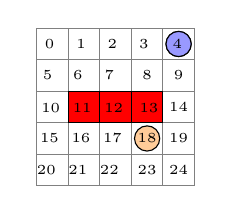
\begin{tikzpicture}[scale=0.8]
\draw[step=0.5cm,color=gray] (-1.5,-1.5) grid (1,1);
\filldraw[fill=blue,draw=black] (+0.75,+0.75) circle (0.2cm);
\filldraw[fill=red,draw=black] (0,0) rectangle (-0.5,-0.5);
\filldraw[fill=red,draw=black] (-0.5,0) rectangle (-1,-0.5);
\filldraw[fill=red,draw=black] (0,0) rectangle (0.5,-0.5);
\filldraw[fill=blue!40!white,draw=black] (+0.75,+0.75) circle (0.2cm);
\filldraw[fill=orange!40!white,draw=black] (0.25,-0.75) circle (0.2cm);
\node at (-1.30,+0.75) {\tiny{0}};
\node at (-0.80,+0.75) {\tiny{1}};
\node at (-0.30,+0.75) {\tiny{2}};
\node at (0.20,+0.75) {\tiny{3}};
\node at (0.73,+0.75) {\tiny{4}};
\node at (-1.33,+0.25) {\tiny{5}};
\node at (-0.85,+0.25) {\tiny{6}};
\node at (-0.35,+0.25) {\tiny{7}};
\node at (0.25,+0.25) {\tiny{8}};
\node at (0.75,+0.25) {\tiny{9}};
\node at (-1.28,-0.27) {\tiny{10}};
\node at (-0.78,-0.27) {\tiny{11}};
\node at (-0.28,-0.27) {\tiny{12}};
\node at (0.28,-0.27) {\tiny{13}};
\node at (0.75,-0.25) {\tiny{14}};
\node at (-1.3,-0.75) {\tiny{15}};
\node at (-0.8,-0.75) {\tiny{16}};
\node at (-0.3,-0.75) {\tiny{17}};
\node at (0.25,-0.75) {\tiny{18}};
\node at (0.75,-0.75) {\tiny{19}};
\node at (-1.35,-1.25) {\tiny{20}};
\node at (-0.85,-1.25) {\tiny{21}};
\node at (-0.35,-1.25) {\tiny{22}};
\node at (0.25,-1.25) {\tiny{23}};
\node at (0.75,-1.25) {\tiny{24}};
\end{tikzpicture}
\hspace{.3cm}}
%\hfill
\subfloat[Transitions from the initial state\label{fig:simple-transitions}]{
\begin{minipage}{5.0cm}
\vspace{-1.8cm}
{\fontsize{8}{10}\selectfont $\vis(4,18) = \false,\vis(4,17) = \false,$ $\vis(4,19) = \true, \vis(4,23) = \false$}

\smallskip

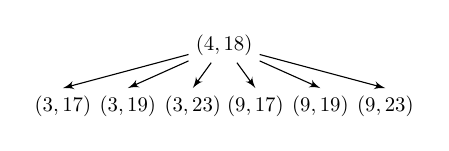
\begin{tikzpicture}[node distance=.75 cm,auto,>=latex',line join=bevel,transform shape,scale=0.75]
\node at (0,0) (s0) {$(4,18)$};
\node  [below left of=s0,yshift=-.5cm] (s3) {$(3,23)$};
\node  [below right of=s0,yshift=-.5cm] (s4) {$(9,17)$};
\node  [left of=s3,xshift=-.35cm] (s2) {$(3,19)$};
\node  [left of=s2,xshift=-.35cm] (s1) {$(3,17)$};
\node  [right of=s4,xshift=.35cm] (s5) {$(9,19)$};
\node  [right of=s5,xshift=.35cm] (s6) {$(9,23)$};

\draw [->] (s0) edge (s1.north);
\draw [->] (s0) edge (s2.north);
\draw [->] (s0) edge (s3.north);
\draw [->] (s0) edge (s4.north);
\draw [->] (s0) edge (s5.north);
\draw [->] (s0) edge (s6.north);
\end{tikzpicture}
\end{minipage}

}

\caption{A simple surveillance game on a grid arena. Obstacles are shown in red, the agent (at location 4) and the target (at location 18) are coloured in blue and orange respectively.}
\label{fig:simple-surveillance-game}

\end{figure}


The transition relation $\delta$ encodes the one-step move of both the target and the agent, where the target moves first and the agent moves second. For a state $(l_a,l_t)$ we define $\succs_t(l_a,l_t)$ as the set of successor locations of the target.

\begin{example}\label{ex:simple-surveillance-game}
Figure~\ref{fig:simple-surveillance-game} shows an example of a surveillance game on a grid.  The sets of possible locations $L_a$ and $L_t$ for the agent and the target consist of the squares of the  grid. The transition relation $\delta$ encodes the possible one-step moves of both the agent and the target on the grid, and incorporates all desired constraints. For example, moving to an occupied location, or an obstacle, is not allowed. Figure~\ref{fig:simple-transitions} shows the possible transitions from the initial state $(4,18)$.

The function $\vis$ encodes straight-line visibility: a location $l_t$ is visible from a location $l_a$ if there is no obstacle on the straight line between them. Initially the target is not in the area of sight of the agent, but the agent knows the initial position of the target. However, once the target moves to one of the locations reachable in one step, in this case, locations $\{17,19,23\}$, this might no longer be the case. More precisely, if the target moves to location $19$ (by choosing $\sigma_i = W$), then the agent observes its location, but if it moves to one of the others, then the agent no longer knows its exact location.
\end{example}



\subsection{Belief-Set Game Structures}

For surveillance games, when the target is not in vision, it is natural that we need reason about the \emph{belief} the agent has in the location of the target. 
 To this end, we can employ a powerset construction which is commonly used to transform a partial-information game into a perfect-information one, by explicitly tracking the knowledge one player has as a set of possible states of the other player.

Given a set $B$, we denote with $\mathcal{P}(B) = \{B' \mid B'\subseteq B\}$ the powerset (set of all subsets) of $B$.

For a surveillance game structure $G = (\game,\vis)$ we define the corresponding \emph{belief-set game structure} $G_\belief  = (\game_\belief,\vis)$ where $\game_\belief = (\states_\belief,s^\init_\belief,\alphabet,\delta_\belief)$ with the following components:
\begin{itemize}
\item $\states_\belief = L_a \times \beliefs$ is the set of states, with $L_a$ the set of locations of the agent, and $\beliefs$ the set of \emph{belief sets} describing information about the location of the target;
\item $s^\init_\belief = (l_a^\init,\{l_t^\init\})$ is the initial state;
\item $\alphabet$ is the same as given in the underlying surveillance game;
\item $\delta_\belief: \states_\belief \times \ialphabet \rightarrow \states_\belief \times \states_\belief$ is the transition relation.
\end{itemize}
\begin{figure}
\begin{center}
\vspace{0.2cm}
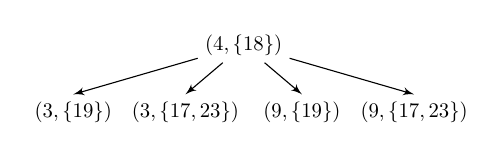
\begin{tikzpicture}[node distance=.9 cm,auto,>=latex',line join=bevel,transform shape,scale=.75]
\node at (0,0) (s0) {$(4,\{18\})$};
\node  [below left of=s0,yshift=-.5cm,xshift=-.35cm] (s2) {$(3,\{17,23\})$};
\node  [below right of=s0,yshift=-.5cm,xshift=.35cm] (s3) {$(9,\{19\})$};
\node  [left of=s2,xshift=-1cm] (s1) {$(3,\{19\})$};
\node  [right of=s3,xshift=1cm] (s4) {$(9,\{17,23\})$};

\draw [->] (s0) edge (s1.north);
\draw [->] (s0) edge (s2.north);
\draw [->] (s0) edge (s3.north);
\draw [->] (s0) edge (s4.north);
\end{tikzpicture}
\end{center}



\caption{Transitions from the initial state in the belief-set game from Example~\ref{ex:simple-belief-game} where $\vis(4,17) = \vis(4,23) = \false$.}
\label{fig:simple-belief-game}

\end{figure}

\begin{example}\label{ex:simple-belief-game}
Consider the surveillance game structure from Example~\ref{ex:simple-surveillance-game}. The initial belief set is $\{18\}$, consisting of the target's initial position. After the first move of the target, there are two possible belief sets: the set $\{19\}$ resulting from the move to a location in the area of sight of the agent, and $\{17,23\}$ consisting of the two invisible locations reachable in one step from location $18$.
Figure~\ref{fig:simple-belief-game} shows the successor states of the initial state $(4,\{18\})$ in $G_\belief$. 
\end{example}

A \emph{run} in the game $G_\belief$ is an infinite sequence $s_0,s_1,\ldots$ of states in $\states_\belief$, where $s_0 = s_\belief^\init$,  $\delta_\belief(s_i,\sigma) = s_{i+1}$ for all $i$. 

A \emph{strategy for the target in $G_\belief$} is a function $f_t: \states_\belief \to \beliefs$ such that a strategy for the target suggests a move resulting in some belief set reachable from some location in the current belief.

A \emph{strategy for the agent in $G_\belief$} is a function $f_a : S_\belief \times \beliefs \to S_\belief$. Intuitively, a strategy for the agent suggests a move based on the observed history of the play and the current belief about the target's position.

The outcome of given strategies $f_a$ and $f_t$ for the agent and the target in $G_\belief$, denoted $\outcome(G_\belief,f_a,f_t)$, is a run $s_0,s_1,\ldots$ of $G_\belief$ such that for every $i \geq 0$, we have $s_{i+1} = f_a(s_0,\ldots,s_i,B_t^i)$, where $B_t^i = f_t(s_0,\ldots,s_i)$.


\subsection{Temporal Surveillance Objectives}
Since the states of a belief-set game structure track the information that the agent has, we can state and interpret surveillance objectives over its runs. We now formally define the surveillance properties in which we are interested. 

We consider a set of \emph{surveillance predicates} $\SP = \{p_k \mid k \in \nats_{>0}\}$, where for $k \in \nats_{>0}$ we say that a state $(l_a,B_t)$ in the belief game structure satisfies $p_k$ (denoted $(l_a,B_t) \models p_k$) iff 
$|\{l_t \in B_t \mid \vis(l_a,l_t)  = \false \}| \leq k$. Intuitively, $p_k$ is satisfied by the states in the belief game structure where the size of the belief set does not exceed the threshold $k \in \nats_{>0}$.

We study surveillance objectives expressed by formulas of linear temporal logic (LTL) over surveillance predicates.
% Since we are only interested in surveillance predicates that upper-bound the size of belief sets, we consider LTL formulas in negation normal form, in which we disallow the occurrence of negation in front of surveillance predicates.
 The LTL surveillance formulas  are generated by the grammar\\
$\varphi := p \mid \true \mid \false \mid \varphi \wedge \varphi \mid \varphi \vee \varphi \mid \LTLnext  \varphi  \mid \varphi \LTLuntil \varphi \mid \varphi \LTLrelease \varphi,$\\
where $p \in \SP$ is a surveillance predicate, $\LTLnext$ is the \emph{next} operator, $\LTLuntil$ is the \emph{until} operator, and $\LTLrelease$ is the \emph{release} operator. We also define the derived operators 
\emph{finally}: $\LTLfinally \varphi = \true \LTLuntil \varphi$ and 
\emph{globally}: $\LTLglobally \varphi = \false \LTLrelease \varphi$.

LTL formulas are interpreted over (infinite) runs. If a run $\rho$ satisfies an LTL formula $\varphi$, we write $\rho \models \varphi$. The formal definition of LTL semantics can be found in~\cite{BaierKatoen08}. Here we informally explain the meaning of the formulas we use.

Of special interest will be surveillance formulas of the form $\LTLglobally p_k$, termed \emph{safety surveillance objective}, and $\LTLglobally\LTLfinally p_k$, called \emph{liveness surveillance objective}.
Intuitively, the safety surveillance formula $\LTLglobally p_k$ is satisfied if at each point in time the size of the belief set does not exceed $k$. The liveness surveillance objective $\LTLglobally\LTLfinally p_k$, on the other hand, requires that infinitely often this size is below or equal to $k$.


\subsection{Surveillance Synthesis Problem}
A \emph{surveillance game} is a pair $(G,\varphi)$, where $G$ is a surveillance game structure and $\varphi$ is a surveillance objective. A \emph{winning strategy for the agent for $(G,\varphi)$} is a strategy $f_a$ for the agent in the corresponding belief-set game structure $G_\belief$ such that for every strategy $f_t$ for the target in $G_\belief$ it holds that $\outcome(G_\belief,f_a,f_t) \models \varphi$. Analogously, a \emph{winning strategy for the target for $(G,\varphi)$} is a strategy $f_t$ such that, for every strategy $f_a$ for the agent in $G_\belief$, it holds that $\outcome(G_\belief,f_a,f_t) \not\models \varphi$.
A \emph{permissive} winning strategy for the agent $f_s$ is a strategy that is not only winning for the agent, but also contains all deterministic winning strategies.

{\bf Surveillance synthesis problem:} Given a surveillance game $(G,\varphi)$, compute a permissive winning strategy for the agent for $(G,\varphi)$, or determine that such a strategy does not exist.


It is well-known that two-player perfect-information games with LTL objectives over finite-state game structures are determined, that is exactly one of the players has a winning strategy~\cite{BorelDeterminacy}. This means that the agent does not have a winning strategy for a given surveillance game, if and only if the target has a winning strategy for this game. We refer to winning strategies of the target as \emph{counterexamples}.

We note that to avoid the state space blow up arising from the subset construction, we can solve these games using the techniques outlined in \cite{Bh2018}

\section{Patrol}


Let $\mathcal{X}$ be the set of all possible environment configurations.
Each $\Omega \in \mathcal{X}$ is an open set representing the free space
and $\Omega^C$ is a closed set consisting of a finite number of connected components.
Let $\mathcal{O} = \{x_i\}_{i=0}^k$ be the sequence of vantage points. For
each vantage point, the operator $\proj_{x_i}\Omega$ is a projection of
$\Omega$ along $x_i$. Then $\proj_{x_i}\Omega$ is a set of range measurements defined
on the unit sphere.  The back projection $\backproj$ maps the range
measurements to the visibility set
$\mathcal{V}_{x_i} \Omega := \backproj (\proj_{x_i}) \Omega$;
that is, points in this set are visible from $x_i$.
As more range measurements are acquired, the
environment can be approximated by the \emph{cumulatively visible set} $\Omega_k$:
$$\Omega_k = \bigcup_{i=0}^k \mathcal{V}_{x_i}\Omega \ . $$

By construction, $\Omega_k$ admits partial ordering: $\Omega_{i-1} \subset \Omega_{i}$.
For suitable choices of $x_i$, it is possible that $\Omega_n \to \Omega$,
(say, in the Hausdorff distance).  We aim at determining a \emph{minimal number
of  vantage points}  from which every point in $\Omega$ can be seen.


\subsection{A Greedy Approach}
We consider a greedy approach which sequentially determines a new vantage point, $x_{k+1}$, based on the information gathered from all previous vantage points, $x_0,x_1,\cdots, x_{k}$.
The strategy is greedy because $x_{k+1}$ would be a location that \emph{maximizes the information gain}.

If the environment $\Omega$ is known, we define the \emph{gain} function
$$g(x;\Omega_k, \Omega) := |   \mathcal{V}_x \Omega \cup \Omega_k| - |\Omega_k |, $$

i.e. the volume of the region that is visible from $x$ but not from $x_0,x_1,\cdots,x_{k}$. 

Define $\Gamma$ as the feasible set (satisfying the surveillance requirements).
Then, for patrolling, we consider:
\begin{equation} x_{k+1} = \arg \max_{x\in \Gamma} g(x;\Omega_k, \Omega).\end{equation}
In other words, the next vantage point should be the point in the feasible set that maximizes the newly surveyed area. 

\section{Surveillance game abstraction}

\section{Experimental evaluation}

\section{Conclusion}

\bibliographystyle{IEEEtran}
\bibliography{main}

\end{document}
